\documentclass[11pt]{article}
    \title{%
        CropFactorCalculator\\
        \large En räknare för fotografer}
    \author{Nils Korsfeldt}
    \date{Februari 2021}

    % General document formatting
    \usepackage[english]{babel}
    \usepackage[margin=1in]{geometry}
    \usepackage[parfill]{parskip}
    \usepackage[utf8]{inputenc}

    \usepackage[usestackEOL]{stackengine}
    \usepackage{outlines}
    \usepackage{blindtext, color, soulutf8}
    \usepackage[usestackEOL]{stackengine}
    \usepackage[document]{ragged2e}
    \usepackage{microtype}
    \usepackage{hyperref}
    \usepackage[countmax]{subfloat}

    \usepackage{graphicx}
    \graphicspath{ {./img/} }

    % Related to math
    \usepackage{amsmath,amssymb,amsfonts,amsthm}

\begin{document}

\maketitle

{\raggedleft\vfill{%
    Nils Korsfeldt \\ 
    Gymnasiearbete 100 poäng \\
    Klass 17ts \\
    Teknikprogrammet \\
    Läsåret 2019/2020 \\
    Handledare: Bondhon Shahriar Alam
}\par
}

\clearpage

\begin{abstract}
\normalsize

% Abstracts in Swedish and English, not sure which one to use so ask Bond

% Swedish
\iffalse 0
Denna rapport redogör för framtagandet samt utvecklingen av ett verkyg för att
räkna ut beskärningsfaktor/förlängningsfaktor för fotografi på olika format.
Rapporten omfattar vad som ledde till utvecklingen av denna, samt hur den skulle
kunna appliceras i professionella situationer och amatörsituationer. Den jämför
också verktyget med liknande verktyg som redan finns.\par
\bigskip

Undersökningen har utförts i form av intervjuer med bekanta fotointresserade och
utifrån det har det tagits fram en uppfattning om efterfrågan för verktyget.
Undersökningen har även kollat på vad verktyget kan erbjuda i jämförelse med
sina konkurrenter, detta förklaras vidare i sektion 2 och 3.
\fi

% English
This report accounts for the development of a tool that is used to calculate
crop factors when doing cross-format photography. The report covers what led to
the development of this tool, and how it could be used in professional
situations as well as amateur ones. It also compares the tool to other similar
tools that already exist.\par
\bigskip

The survey has been performed in the form of short discussions with fellow
individuals interested in photography, and the interest for this tool has been 
gauged based on that. The analysis has also looked at what the tool can offer
in comparison to it's "competitors", this is further covered in
sections 2 and 3.

\end{abstract}

\clearpage

\renewcommand{\contentsname}{Innehållsförteckning}
\tableofcontents

\clearpage

\section{Inledning}
Om du någonsin har använt kameror med olika sensorformat eller filmformat så
har du kanske stött på problemet att konvertera brännvidder och bländare
mellan dessa, eller, exempelvis, att jämföra ett objektiv på en sensor med
samma objektiv på en annan sensor som är större eller mindre.\par

Den grundläggande matematiken är som följande:\par

Låt A vara sensorn på referenskameran och B vara sensorn på kameran vi
räknar för, samt låt W beteckna bredd och H beteckna höjd.

\[
\frac{ \sqrt{ \text{A}_W^2 + \text{A}_H^2 } }
     { \sqrt{ \text{B}_W^2 + \text{B}_H^2 } }
     = \text{beskärningsfaktor} 
\]

För den som har svårt att läsa det ovanstående så är det grundläggande logisk
aritmetik med Pythagoras sats i fokus; sammanfattat så räknar vi ut diagonalerna
på sensorn i vår referenskamera och sensorn i kameran vi ska använda och delar
sedan dem med varandra. Vi får då ut en faktor, som objektivets brännvidd och
bländare multipliceras med.\par

Ett exempel:\par

Låt vår referenskamera ha en sensorstorlek på 36x24mm och kameran vi
ska använda ha en sensorstorlek på 23.7x15.6mm (APS-C). Objektivet vi använder
har en brännvidd på 50mm och en bländare på f/1.8.

\begin{equation}
\frac{ \sqrt{36^2 + 24^2 } }
     { \sqrt{23.7^2 + 15.6^2 } }
     \approx \frac{43.27}{28.37}
     \approx 1.53
\end{equation}

Vår beskärningsfaktor blir alltså ca 1.53, och vi får det följande om vi
applicerar detta på vårt objektiv (som specificerat ovan).

\begin{equation}
    50 \cdot 1.53 = 76.5 \ \text{(mm)}
\end{equation}
\begin{equation}
    1.8 \cdot 1.53 \approx \text{(f/)} 2.75
\end{equation}

Resultatet blir att vårt objektiv, som är ett 50mm f/1.8 på en 36x24mm sensor
kommer att motsvara ett 76.5mm f/2.75 på en 23.7x15.6mm sensor.

\bigskip
I detta projekt siktar jag på att lösa detta problem med ett enkelt verktyg som
låter en jämföra sensorer och brännvidder som förklarat. Jag har valt detta för
att jag är insatt i fotografi och har haft just det här problemet flera gånger,
samt för att jag tycker att själva tekniken bakom fotografi och filmografi är
intressant.\par

\section{Syfte och frågeställningar}
Syftet med detta arbete är att utreda varför det finns ett behov
för ett nytt verktyg som räknar ut beskärningsfaktor/förlängningsfaktor, samt
hur detta nya verktyg presterar i jämförelse med de som redan finns "på
marknaden". Med prestation menas hur funktionellt verktyget, hur lätt/intuitivt
det är att använda, samt hur bra information det ger som output.

Frågeställningen är som följande:\par

\begin{enumerate}
    \item Hur skulle detta verktyg kunna appliceras i professionellt arbete/en
        professionell situation? Det vill säga, hur skulle en professionell
        fotograf eller fotostudio kunna använda detta verktyg i sitt
        arbetsflöde?
    \item Vad uppmanade utvecklingen av detta verktyg och hur skiljer verktyget
        sig från sina konkurrenter? Orsak bakom framtagandet, fördelar och
        nackdelar gentemot liknande verktyg.
\end{enumerate}

\section{Material och metod}
\sloppy
För att få svar på dessa frågor har det utförts intervjuer (läs: Sektion 4.1)
med vänner som också är fotointresserade. Vännerna i fråga är Jacob Nilsson
Lehmusjärvi och Daniel Stridh. Båda har tagit examen i estet med fotografisk
inriktning från NTI-Gymnasiet Stockholm och de anses av författaren vara
pålitliga källor med väl grundade åsikter och uttalanden i ämnet. Intervjuerna
har utförts över chattapplikationen Discord i stället för personligen, med 
respekt till de rådande omständigheterna gällande COVID-19.\par

De följande frågorna har ställts: 
\fussy

\begin{itemize}
    \item Fråga 1: Vilken roll spelar fotografi i ditt vardagsliv?
    \item Fråga 2: Har du stött på problemet i fråga?
    \item Fråga 3: Skulle du använda detta verktyg om det fanns?
\end{itemize}

\bigskip

Utöver detta så har verktyget jämförts med liknande verktyg som redan finns. Det
som har jämförts är vilken input/output som finns tillgängliga, samt hur
informativt och intuitivt detta är att använda/läsa. I undersökningen finns
skärmbilder av verktygen samt en skriftlig överblick över vilken funktionalitet
som till synes finns tillgänglig för respektive verktyg.\par

\sloppy
Verktyget som har nämnts flera gånger i denna rapport,
\emph{CropFactorCalculator}, är en hemsida som har byggts i ramverket ReactJS,
som fungerar på det sättet att det förvandlar HTML-taggar till något mer
abstrakt, nämligen en Javascript-funktion. Detta tillåter att man kan konstruera
egna "komponenter", som är en grupp av element, genom att skriva funktioner för
dem. Dessa komponenter skriv i separata filer, och inkluderas med
\texttt{import} varpå de kan anropas med vanlig HTML-syntax
(e.g. \texttt{<MinKomponent>}). HTML-egenskaper som komponenten anropas med kan
kommas åt i funktionen genom variabeln \texttt{props}. Funktionen returnerar
sedan ett HTML-kodblock, som kan innehålla flera element, till och med egna
komponenter (d.v.s. att komponenter kan nästlas). Detta gör att man kan göra, i
praktiken, väldigt avancerade skräddarsydda HTML-element, som dessutom kan
återanvändas. Ett exempel på detta i verktyget är dropdown-menyerna, som läser
in alternativ från en CSV-fil och returnerar en \texttt{<select>} populerad med
\texttt{<option>}s skapade utifrån CSV-filens rader.
\fussy

\clearpage

\section{Undersökning och resultat}
\subsection{Intervjuer}
\subsubsection{Intervjuer - frågor och svar}
\textbf{Vilken roll spelar fotografi i ditt vardagsliv?}\par

Jacob: ”Numera inte så mycket, men förr; jättemycket. Jag tar dock några bilder
per dag med mobilkameran och fotar ibland med en "riktig" kamera, oftast en
analog.”\par

Daniel: ”Vardagsliv är väl lite av en överdrift, men jag är med i
Melodifestivalklubben och fotar ibland för dem på olika evenemang eller
tillställningar. Numera är mitt fotograferande mest förlagt till evenemang men
foto är fortfarande för mig en viktig hobby.”\par

\textbf{Har du stött på problemet i fråga?}\par

Jacob: ”Nej, men det bygger på att jag inte brukar använda exempelvis spegellös
digitalkamera när jag fotar. Dock en tid funderade jag på att skaffa en sådan
just på grund av att man kan använda äldre objektiv på den, eftersom jag redan
har flera. På grund av den ekonomiska faktorn köpte jag inte en.”\par

\sloppy
Daniel: ”Jag har faktiskt köpt ett 50-220mm objektiv till min digitalkamera, men
som egentligen passar ett annat bajonettfäste. Så när jag monterar objektivet
med en adapter så kommer jag att få en annorlunda brännvidd än vad objektivet
skulle ge på fästet det egentligen passar.”\par
\fussy

\textbf{Skulle du använda detta verktyg om det fanns?}\par

Jacob: ”Ja, i det fallet att jag skulle äga en spegellös digitalkamera så
skulle det här nog komma väl till hands för att räkna på hur det skulle fungera
med mina gamla objektiv.”\par

Daniel: ”När mitt objektiv kommer fram så kommer jag nog att använda det, ja.”
\par


\subsubsection{Sammanfattning}
\sloppy
Jacob har ett tydligt fotointresse och fotar ibland med analoga kameror, men
annars oftas med mobilen. Han var ett tag inne på att köpa en spegellös
digitalkamera som han skulle kunna sätta sina äldre objektiv på. Han säger att
om han hade gjort det så skulle verktyget komma till användning.\par

Daniel har ett likvärdigt fotointresse och fotar ibland på evenemang som press.
Han har köpt ett nytt objektiv till sin digitalkamera som passar ett annat
fäste, och när han använder en adapter så kommer han att få en annan brännvidd.
Han säger att när hans objektiv kommer fram så kommer han nog[sic] att använda
verktyget. \par
\fussy

\clearpage

\subsection{Jämförelse med liknande verktyg}
\subsubsection{Skärmdumpar}
\renewcommand{\figurename}{Fig.}

\begin{subfigures}

\begin{figure}[!htb]
\caption{CropFactorCalculator, input}
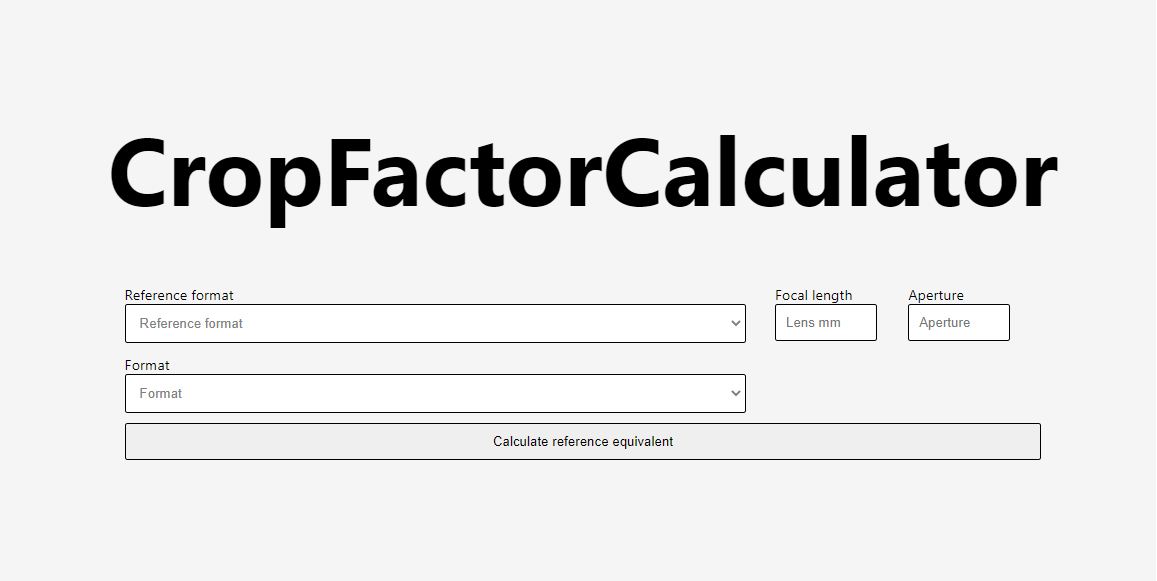
\includegraphics[width=\textwidth]{cfc-in}
\end{figure}

\begin{figure}[!htb]
\caption{CropFactorCalculator, exempel på output}
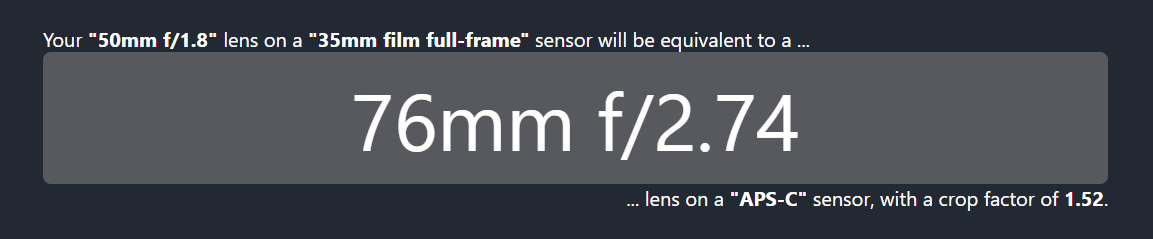
\includegraphics[width=\textwidth]{cfc-out}
\end{figure}

\end{subfigures}

\begin{subfigures}

\begin{figure}[!htb]
\caption{CropFactorCalculator}
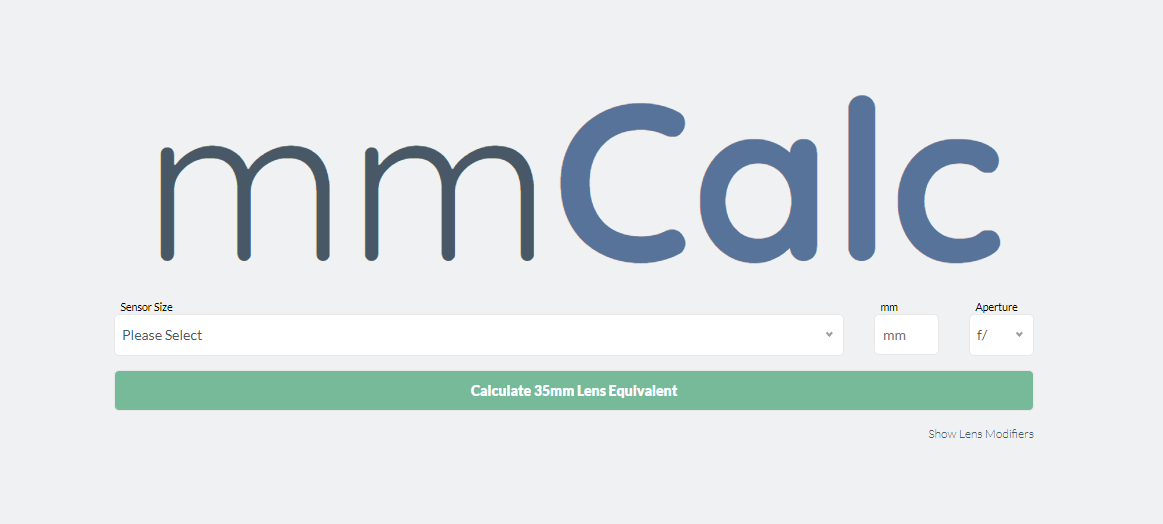
\includegraphics[width=\textwidth]{mmcalc-in}
\end{figure}

\begin{figure}[!ht]
\caption{CropFactorCalculator}
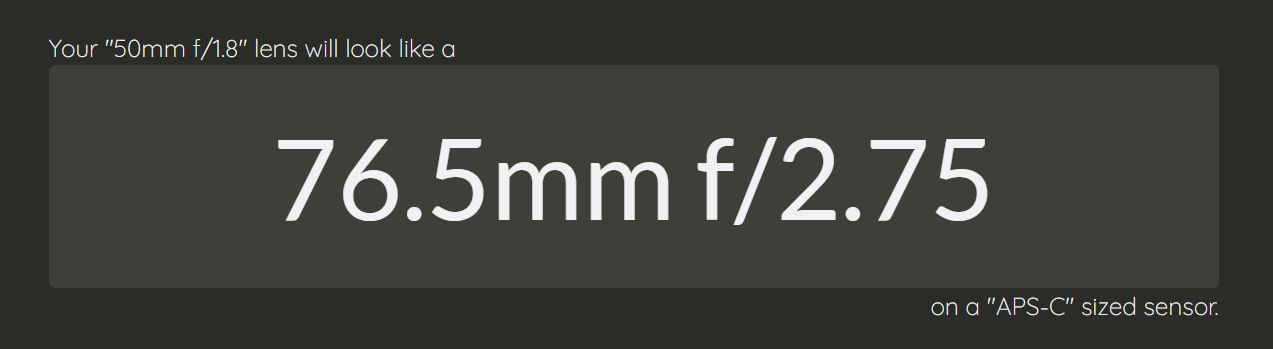
\includegraphics[width=\textwidth]{mmcalc-out}
\end{figure}

\end{subfigures}

\clearpage

\subsubsection{Sammanfattning}
\sloppy
I figur 1a, som visar input-formuläret för \emph{CropFactorCalculator}, kan vi
se att det finns fält för referensformat ("Reference format"), format
("Format"), brännvidd ("Focal length"), och bländare ("Aperture"). I figur 1b,
som visar exempel på output från \emph{CropFactorCalculator}, kan vi se att man
får information om referensformat, format och resulterande bränndvidd respektive
bländartal.\par

I figur 2a, som visar input-formuläret för \emph{mmCalc}, kan vi se att det
finns fält för format ("Sensor size"), brännvidd ("mm"), och bländare
("Aperture"). I figur 2b, som visar exempel på output från \emph{mmCalc}, kan vi
se att man får information om objektivet, format samt resulterande brännvidd
respektive bländartal.\par
\fussy

\section{Analys och diskussion}
\subsection{Allmän analys/diskussion}
\sloppy
Intervjuobjekten har ett vardagligt intresse för fotografi, både som hobby och
mer professionellt. De har därför varit relevanta att fråga för att de har
tidigare kunskap i området. Dessutom så har de, som sagt, tagit examen från
NTI-Gymnasiet Stockholm inom estet med fotografisk inriktning. \par

Eftersom att de har visat intresse för verktygen så anser jag att det finns en
rimlig anledning att utveckla det. De båda skulle använda verktyget för att
förenkla sitt arbete inom fotografi. Jacob skulle kunna använda det om han hade
köpt en digitalkamera som han kan använda sina gamla objektiv på. I det fallet
att han söka jobb som exempelvis porträttfotograf skulle allt detta gå bra ihop;
gamla objektiv används ofta av porträttfotografer för de speciella effekter som
de ger. Även Daniel, som faktiskt har köpt ett nytt objektiv, kommer att kunna
få nytta av verktyget när han ska använda objektivet på sin digitalkamera. Detta
kommer att vara relevant i den professionella situationen att han fotar på
evenemang för exempelvis Melodifestivalklubben.\par

Det som har uppmanat utvecklingen av detta verktyg är att jag själv har stött på
problemet som det löser; att använda ett objektiv som egentligen inte passar på
en kamera och försöka lista ut vilken brännvidd och bländare man kommer få.
Att göra detta manuellt med en miniräknare är ett grovgöra, och en räknare
underlättar massivt.\par

\subsection{Fördelar och nackdelar}
Det finns en "konkurrent" till mitt verktyg som jag känner till, och det är
\emph{mmCalc}.\footnote{mmcalc.com} Jag brukade använda \emph{mmCalc} tills
jag kände att den inte räckte för mina behov längre. Detta leder oss till den
största {(första?)} fördelen som verktyget jag själv utvecklat har, och det
är att det går att ändra referensformatet. På \emph{mmCalc} är
referensformatet låst på 35mm (36x24mm) vilket naturligtvis försvårar om man
ska använda sitt objektiv på något annat än en kamera med den sensorstorleken.
För att förenkla; det enda som kan räknas ut på \emph{mmCalc} är
35mm-motsvarigheten till ens objektiv. På mitt verktyg går det däremot att välja
vilket referensformat som helst, så om du exempelvis ska använda ett objektiv
för 35mm-sensorer på en kamera med en APS-sensor så går det utan problem att
räkna på. \par
En annan, mindre fördel är att det steglöst går att steglöst
specificera bländartal. På \emph{mmCalc} finns det endast ett fast antal
bländartal att välja på, mellan f/0.7 och f/32. En slutgiltig, mindre fördel
som även är en nödvändig funktion med tanke på att verktyget är mer avancerat
är att man i output-fönstret får mer information om uträkningen man har gjort.
\par

En nackdel, dock, är att det inte går att välja telekonverter eller 
vidvinkelkonverter i mitt verktyg. Dessa innebär ett tillbehör som skruvas
fast mellan kameran och objektivet, som kan antingen förlänga (tele) eller
förkorta (vidvinkel) brännvidden. Detta är användbart om man har ett ett fast
objektiv men vill ha det mer/mindre inzoomat.\footnote{Poggers is not academic
language}\par

\bigskip
\fussy

\bigskip
\bigskip
\bigskip
\bigskip

% Notes
\fbox{%
\parbox{400pt}{

\hl{Anteckningar, ignorera:}\par
\title{Problem}
\begin{outline}
    \1 Läsa CSV till json genom react
        \2 Blobs
    \1 API requests till backend
        \2 Lokal testing - browser requests till localhost bryter mot no-cors
        \2 Lösning: tog bort backend
    \1 eval() = farligt
\end{outline}
\bigskip
\title{Todo}
\begin{outline}
    \1 Utveckla undersökning, gör fler intervjuer
    \1 Utveckla frågorna i frågeställningen *
    \1 Utveckla metoder
    \1 Fixa inledningen *
\end{outline}

}%
}
\end{document}
